\documentclass[aps,prb,onecolumn,nofootinbib,superscriptaddress]{revtex4-2}
\usepackage{amsmath,amssymb,amsthm,mathtools,bm}
\usepackage{booktabs}
\usepackage[colorlinks=true,linkcolor=blue,citecolor=blue,urlcolor=blue]{hyperref}
\usepackage{microtype}
\usepackage{graphicx}
\usepackage{placeins}
\graphicspath{{figures/}}
\newcommand{\Id}{\mathbf{1}}
\newcommand{\tr}{\operatorname{tr}}
\newcommand{\Tr}{\operatorname{Tr}}
\newcommand{\ee}{\mathrm e}
\newcommand{\ii}{\mathrm i}
\newcommand{\EntropyCoefficient}{1.0000072}
\newcommand{\ChargeCoefficient}{0.9989488}
\newcommand{\EntropyResidual}{4.18\times10^{-7}}
\newcommand{\ChargeResidual}{9.56\times10^{-6}}
\newcommand{\LeftSlope}{0.1666233}
\newcommand{\RightSlope}{0.1666233}
\newcommand{\LeftWeight}{0.4998699}
\newcommand{\RightWeight}{0.4998699}
\newcommand{\CorrelationBeta}{22.7291}
\newcommand{\CorrelationRSquared}{-0.9234}
\newcommand{\CotExponent}{1.0004103}
\newcommand{\RetainedTopological}{30}
\newcommand{\RetainedTrivial}{28}
\newcommand{\RegulatedGap}{1.41074\times10^{-7}}
\newcommand{\PeriodicGap}{1.50222\times10^{-9}}

\begin{document}
\typeout{BENCHMARK-TEXTWIDTH=\the\textwidth}
\title{Parent Hamiltonian Benchmark Figs}
\author{Asadullah Bhuiyan}
\noaffiliation
\date{October 2026}
\begin{abstract}
We construct deterministic equilibrium benchmarks for the figures of the current
adaptive-circuit manuscript. The reference is the clean signed sum of normalized,
hard-wall-truncated overcomplete Wannier projectors, at range
$n_{\mathrm{shell}}=1$ and exterior parameter $\alpha_2=30$, with periodic boundary
conditions and exact half filling. Nine figure groups reproduce the selected
observables: the local Chern marker, filtered occupation spectra, the low-energy
gap and mode density, correlations, strip entropy and charge variance, restricted
spectra, wall entropy, modular evolution, and antipodal mutual information. A
separate table gives Chern-number deviations for square systems of lengths
$20,30,40$. The clean parent closely realizes the unit entropy and charge
coefficients and equal half-unit wall contributions. Its strictly periodic
low-energy splitting, finite-ring correlator, and discrete spectral-window counts
also expose differences from the trajectory ensemble. This note is a standalone
benchmark collection; it does not modify the manuscript or its appendixes.
\end{abstract}
\maketitle
\setcounter{tocdepth}{2}
\tableofcontents

\clearpage
\section{Clean parent, geometry, and conventions}
\label{sec:construction}
The overcomplete Wannier (OW) modes are generated by the canonical CPU class
\texttt{classA\_U1FGTN}, using its \texttt{construct\_OW\_projectors} method.
For every center, we use the two
$\sigma^x$ trial orbitals and the uniform Bloch projectors at the parameter assigned
to that center. We retain the square support $|d_x|,|d_y|\leq1$, discard support on
the opposite side of a hard wall, and normalize each remaining mode independently.
The lattice is periodic in both directions, with no boundary twist, random mass,
random projector weight, or measurement record. The central slab has parameter
$\alpha_1$ and the exterior has $\alpha_2=30$. Its inclusive coordinates are
\begin{equation}
 x_L=N_x/2-\lfloor N_x/4\rfloor,\qquad
 x_R=N_x/2+\lfloor N_x/4\rfloor.
\end{equation}
Thus the walls are at $(5,15)$ for $N_x=20$ and $(8,22)$ for $N_x=30$.
The exterior connects across the periodic $x$ seam, but all parent matrix elements
between the slab and exterior vanish.

Using the canonical stored OW columns, define the single-particle parent
\begin{equation}
 h_{\mathrm{par}}=\sum_{\boldsymbol r,\nu=A,B}
 \left(|W_{\boldsymbol r,\nu,+}\rangle\langle W_{\boldsymbol r,\nu,+}|
       -|W_{\boldsymbol r,\nu,-}\rangle\langle W_{\boldsymbol r,\nu,-}|\right).
 \label{eq:parent}
\end{equation}
This construction is often called the flattened OW parent because its ingredients
come from band projectors. We retain its actual dispersive eigenvalues; we do not
replace its spectrum by $\pm1$. The energy normalization in Eq.~\eqref{eq:parent}
is fixed, with no rescaling to fit circuit data. Translation symmetry along $y$
reduces diagonalization to $N_y$ blocks of size $2N_x$.

There are $2N_xN_y$ physical orbitals. Filling exactly the lowest $N_xN_y$ levels
gives an occupied frame $V$ and spectral projector $P=VV^\dagger$. The canonical
stored-column convention and manuscript correlation convention are related by
\begin{equation}
 G_{ij}=\langle\hat c_i^\dagger\hat c_j\rangle=P_{ji},\qquad G=P^{\mathsf T}.
 \label{eq:convention}
\end{equation}
All Chern and modular-propagation signs use this mapping. Restricted occupations,
entropy, charge variance, and orbital-summed densities are invariant under this
transpose. No average over distinct states is performed. Averages over translated
cuts are exact spatial averages; their spectra coincide by translation symmetry.

Numerically degenerate eigenvalues are grouped within
$10^{-12}\max(1,\|h_{\mathrm{par}}\|)$. At a partially occupied Fermi-level
subspace we first retain momentum eigenstates, resolve transverse position within
each momentum block, and use projected coordinate vectors to break any remaining
ties. The reverse occupation choice is evaluated as a diagnostic. For the square
$L=30,40$ cases, two Fermi-level modes are unresolved at this tolerance. Their
alternative choices change the tabulated bulk Chern number by less than
$10^{-12}$ and the half-strip entropy by less than $3\times10^{-12}$.
At fixed $N_x=20$, the approximately $1.50\times10^{-9}$ occupied-to-empty
splitting is resolved, so no such tie prescription is needed.

\subsection{Relation to the manuscript and numerical statistics}
Figure captions identify the corresponding current manuscript number, independently
of its asset filename. Ground-state calculations replace trajectory ensembles.
There is no trajectory count or sampling standard error. Joint fits give equal
total weight to each size, using the manuscript's displayed coordinates and fit
windows. We report deterministic residuals; a coefficient from a poor fit is not
assigned a physical scaling interpretation. Logarithms are natural throughout.

\clearpage
\section{Bulk topology: manuscript Figure 2(b,c)}
The local marker is evaluated with the same ordinary periodic-coordinate seam as
the manuscript:
\begin{equation}
 C(\boldsymbol r)=2\pi\ii\sum_\mu
 [G X G Y G-G Y G X G]_{\boldsymbol r\mu,\boldsymbol r\mu}.
\end{equation}
Its full-system sum vanishes as a finite commutator trace; this does not set the
bulk topological invariant to zero. The plot displays $\tanh C$ and the saved
data also contain the untransformed marker.

For the three-sector disk estimator, use $x_0=L/2$, $R=0.2L$, the manuscript's
counterclockwise sector boundaries, and minimum-image displacements. The
estimator is
\begin{equation}
 \mathcal C_G=-24\pi\,\operatorname{Im}
 \tr(G_{CA}G_{AB}G_{BC}).
\end{equation}
Every integer $y_0$ is included. Their spread is at floating-point precision and
is not a statistical uncertainty. The equilibrium table replaces the dynamical
cycle-convergence panel rather than assigning fictitious cycles to a ground state.

\begin{figure}[htbp]
\centering
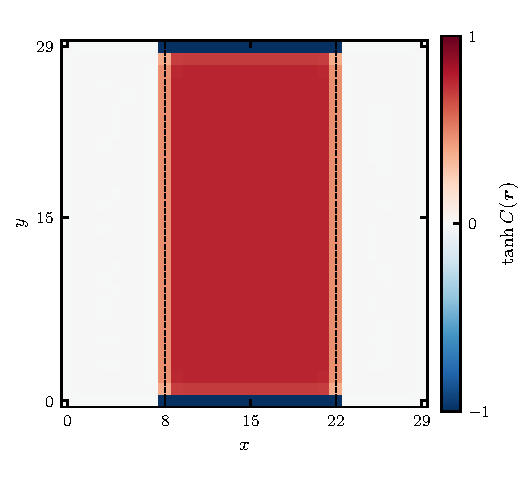
\includegraphics[width=0.5\textwidth]{Parent_02_topology.pdf}
\caption{Ground-state counterpart of manuscript Figure 2(b). Local Chern marker
on the $30\times30$ torus at $\alpha_1=1$, with walls at $x=8,22$.
The color scale is $\tanh C(\boldsymbol r)\in[-1,1]$ and retains the periodic
coordinate seam. There is one clean half-filled ground state and no statistical
averaging.}
\end{figure}
\begin{table}[htbp]
\centering
\setlength{\tabcolsep}{8pt}
\caption{Square-system ground-state counterpart of manuscript Figure 2(c).
The disk centers cover the full circumference.}
\begin{tabular}{rrrrrr}
\toprule
$L$ & $(x_L,x_R)$ & $R$ & $\mathcal C_G$ & $\mathcal C_G-1$ & $|\mathcal C_G-1|$ \\
\midrule
20 & $(5,15)$ & 4 & 0.999957845235 & $-4.215\times10^{-5}$ & $4.215\times10^{-5}$ \\
30 & $(8,22)$ & 6 & 0.999999926439 & $-7.356\times10^{-8}$ & $7.356\times10^{-8}$ \\
40 & $(10,30)$ & 8 & 0.999999999743 & $-2.569\times10^{-10}$ & $2.569\times10^{-10}$ \\
\bottomrule
\end{tabular}

\end{table}

\clearpage
\section{Filtered occupations: manuscript Figure 3(b,c)}
Starting from maximal mixing, imaginary-time filtering with the many-body parent
$\widehat H_{\mathrm{par}}=\sum_{ij}(h_{\mathrm{par}})_{ij}\hat c_i^\dagger\hat c_j$
gives
\begin{equation}
 \hat\rho(t)=\frac{\ee^{-2t\widehat H_{\mathrm{par}}}}
 {\Tr\ee^{-2t\widehat H_{\mathrm{par}}}},\qquad
 n_j(t)=\frac{1}{1+\ee^{2tE_j}},\qquad
 G(t)=\big[\Id+\ee^{2t h_{\mathrm{par}}}\big]^{-\mathsf T}.
 \label{eq:filter}
\end{equation}
This uses the same factor of two as manuscript Eqs.~(13)--(14). We set $t$ to the
numerical values $1,5,60$ of its cycle labels, with no adjustable scale.
Here $t$ is an inverse-energy filtering parameter, not a physical circuit cycle.
The Gaussian state is grand canonical; exact particle-hole pairing fixes its
mean filling to one half. At exactly zero energy, Eq.~\eqref{eq:filter} leaves
occupation $1/2$ even as $t\to\infty$, whereas the separately chosen half-filled
ground state is a projector.

\begin{figure}[htbp]
\centering
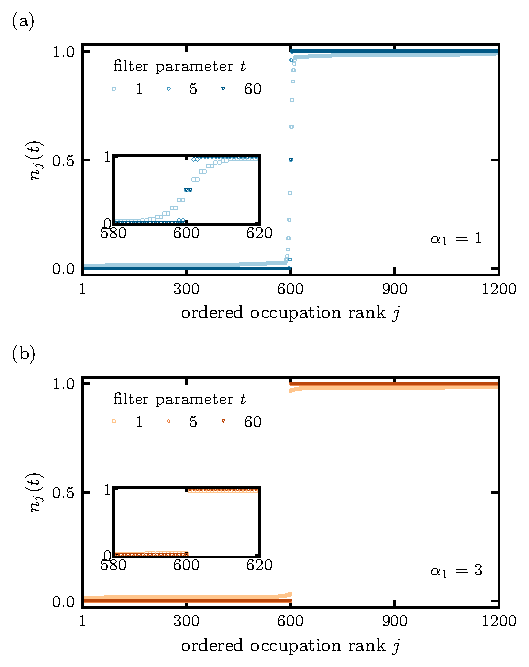
\includegraphics[width=0.5\textwidth]{Parent_03_occupations.pdf}
\caption{Counterparts of manuscript Figure 3(b,c), shown here as panels (a,b).
Ascending filtered occupation spectra at $N_x=20,N_y=30$ for
(a) $\alpha_1=1$ and (b) $\alpha_1=3$, at $t=1,5,60$. All 1200 ranks are shown;
insets use identical limits on ranks $580$--$620$. Eigenvalue ranks are reordered
after applying Eq.~\eqref{eq:filter}. The topological parent retains two
occupations near $1/2$ over these times because its periodic edge splitting is
extremely small. The trivial parent rapidly approaches a projector.}
\end{figure}

\clearpage
\section{Low-energy gap and density: manuscript Figure 4}
Define two distinct spectral gaps:
\begin{equation}
 \delta_{\mathrm{par}}=\min_j|E_j|,\qquad
 g_{\mathrm{hf}}=E_{N_xN_y+1}-E_{N_xN_y}.
\end{equation}
The spectrum is paired, so $g_{\mathrm{hf}}\simeq2\delta_{\mathrm{par}}$.
At fixed $N_x=20$, every circumference in the plotted sweep samples $k_y=0$.
The small interwall hybridization at that momentum controls the minimum gap;
increasing the circumference does not remove it. Thus this clean, periodic
minimum does not reproduce the manuscript's finite-time trajectory-gap
$N_y^{-1}$ trend. We retain the measured values rather than fit them to that law.
This is a boundary-sector and observable distinction, not a failure to construct
the clean topological parent.

The normalized low-energy density is the projector density of all states with
minimum $|E|$, divided by that subspace's dimension. It includes the positive and
negative partners and is independent of their internal basis choice.
\begin{figure}[htbp]
\centering
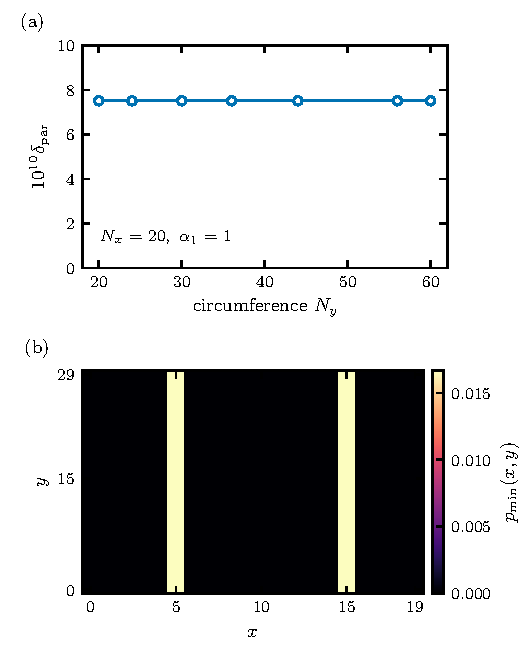
\includegraphics[width=0.5\textwidth]{Parent_04_gap.pdf}
\caption{Counterpart of manuscript Figure 4. (a) Minimum absolute parent energy
at $\alpha_1=1$, fixed $N_x=20$, and $N_y=20,24,30,36,44,56,60$.
The gap remains near $7.5111\times10^{-10}$; connecting lines are guides.
The saved CSV gives both gap definitions and the numerical resolution.
(b) Normalized density of the two minimum-$|E|$ modes at $N_y=30$.
It is uniform along $y$ and concentrated on the two walls.}
\end{figure}

\clearpage
\section{Spatial correlations: manuscript Figure 5}
We retain the manuscript's squared-correlator definition,
\begin{equation}
 C_G(r_y)=\frac{1}{2N_xN_y}\sum_{x,y,\mu,\mu'}
 \left|G_{(x,y,\mu),(x,y+r_y,\mu')}\right|^2,
 \qquad D(\ell)=\frac{N_y}{\pi}\sin\frac{\pi\ell}{N_y}.
\end{equation}
The topological state has much longer-ranged correlations than the trivial state.
However, the periodic clean-parent finite-ring form is not the same as the
trajectory ensemble's antipodally normalized chord power. The same clean
$20\times60$ state was studied in the repository's earlier wall-projected
equilibrium analysis: the wall amplitude fits
$|\cot(\pi r_y/N_y)|^{\eta}$ with $\eta=\CotExponent$ over $5\leq r_y\leq25$.
The squared wall correlator therefore has exponent $2\eta\simeq2$ in that
coordinate. The common-input comparison reproduces the earlier result and is
saved with the source and data hashes.

Near the antipode, the leading cotangent contribution is suppressed. Normalizing
by that small residual amplifies the finite-size differences. Keeping the
requested chord fit gives $\beta=\CorrelationBeta$ with weighted
$R^2=\CorrelationRSquared$; this formal fit is poor and is not evidence for a
large anomalous exponent. The denominator is used as computed, without a floor.

\begin{figure}[htbp]
\centering
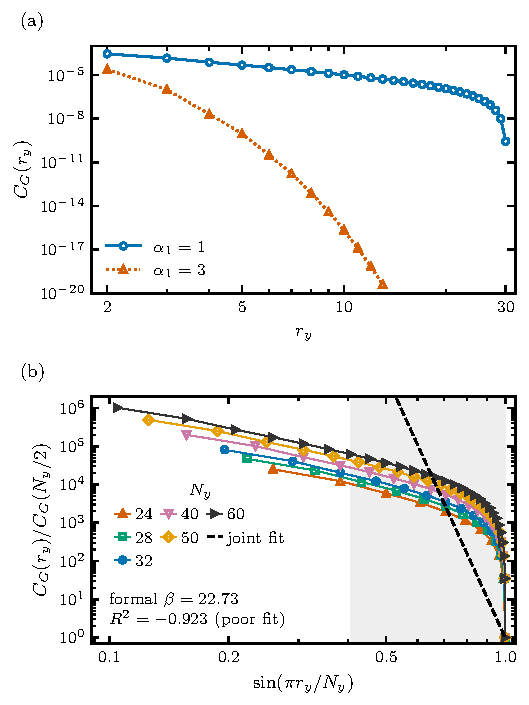
\includegraphics[width=0.5\textwidth]{Parent_05_correlations.pdf}
\caption{Counterpart of manuscript Figure 5. (a) Ground-state squared correlations
at $N_y=60$, comparing $\alpha_1=1,3$, with $N_x=20$. Values at or below
$10^{-20}$ are omitted from this logarithmic display only. (b) Antipodally
normalized $\alpha_1=1$ curves for $N_y=24,28,32,40,50,60$ versus
$\sin(\pi r_y/N_y)$. Displayed separations satisfy $r_y\geq2$; gray shading marks
the union of the $8\leq r_y\leq N_y/2$ fitting windows. The dashed curve is the
requested zero-intercept joint log fit, whose poor residual is explicitly
reported. Its disagreement with the data is part of the benchmark.}
\end{figure}

\clearpage
\section{Strip entropy and charge: manuscript Figure 6}
For a full-width strip of $A_y$ consecutive rows, let $\nu_a$ be the eigenvalues
of $G_A$. We compute
\begin{equation}
 S(A_y)=\sum_a h(\nu_a),\qquad F(A_y)=\sum_a\nu_a(1-\nu_a),\qquad
 h(\nu)=-\nu\log\nu-(1-\nu)\log(1-\nu).
\end{equation}
The exact endpoint limit $0\log0=0$ is used; only roundoff outside $[0,1]$ is
clipped. Subtract the reference at $A_y^*=\lfloor N_y/2\rfloor$ and use
$X=\log[D(A_y)/D(A_y^*)]$, including the same rounded reference for odd sizes.
Joint zero-intercept fits to $\Delta S=(c/3)X$ and
$\Delta F=(k/\pi^2)X$ give
\begin{equation}
 c=\EntropyCoefficient,\qquad k=\ChargeCoefficient.
\end{equation}
The weighted RMS residuals are $\EntropyResidual$ and $\ChargeResidual$,
respectively. These are deterministic fit discrepancies, not standard errors.

\begin{figure}[htbp]
\centering
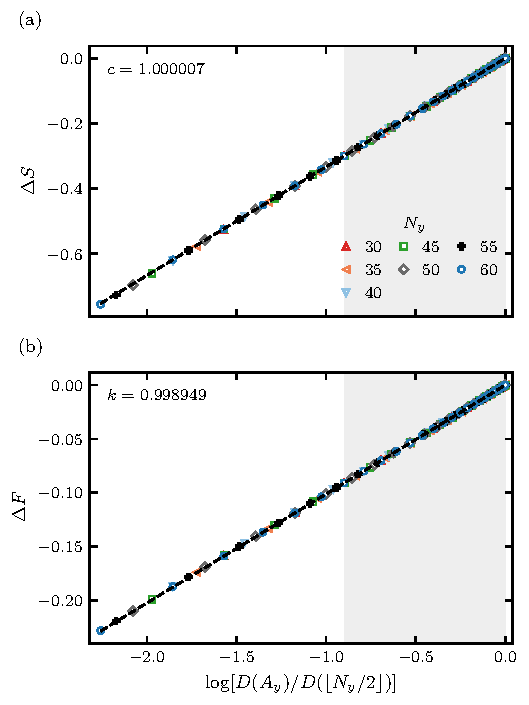
\includegraphics[width=0.5\textwidth]{Parent_06_entropy_charge.pdf}
\caption{Counterpart of manuscript Figure 6. Half-strip-subtracted (a) entropy
and (b) charge variance for $N_y=30,35,40,45,50,55,60$, $N_x=20$, and
$\alpha_1=1$. Points begin at $A_y=2$; fits use
$8\leq A_y\leq\lfloor N_y/2\rfloor$ with equal total weight per size.
Shading marks the union of those fit windows.}
\end{figure}

\clearpage
\section{Restricted spectra: manuscript Figure 7}
The full occupation histogram uses 100 equal bins on $[0,1]$. The conditional
entanglement-energy histogram uses
\begin{equation}
 \varepsilon=\log\frac{1-\nu}{\nu},\qquad
 W:\ |2\nu-1|<0.99,
\end{equation}
and 101 equal bins on $[-\log199,\log199]$. Both densities integrate to one.
At $N_y=32$, every translated half-strip has 640 occupations. There are
\RetainedTopological\ retained levels per cut for $\alpha_1=1$ and
\RetainedTrivial\ for $\alpha_1=3$. Pooling the 32 identical translated spectra
changes counts but not normalized densities; it does not provide independent
samples or smooth a discrete spectrum.

The raw count $N_{0.99}(A_y)$ is an integer staircase. For the clean topological
state it is exactly 30 throughout the prescribed fit window $5\leq A_y\leq16$.
The best affine log-chord fit is therefore constant. Its $R^2$ is undefined
because the total variation is zero. This differs from the smoothly growing
trajectory-averaged count and does not contradict logarithmic entropy: eigenvalues
can move within the fixed window while its count stays constant.

\begin{figure}[htbp]
\centering
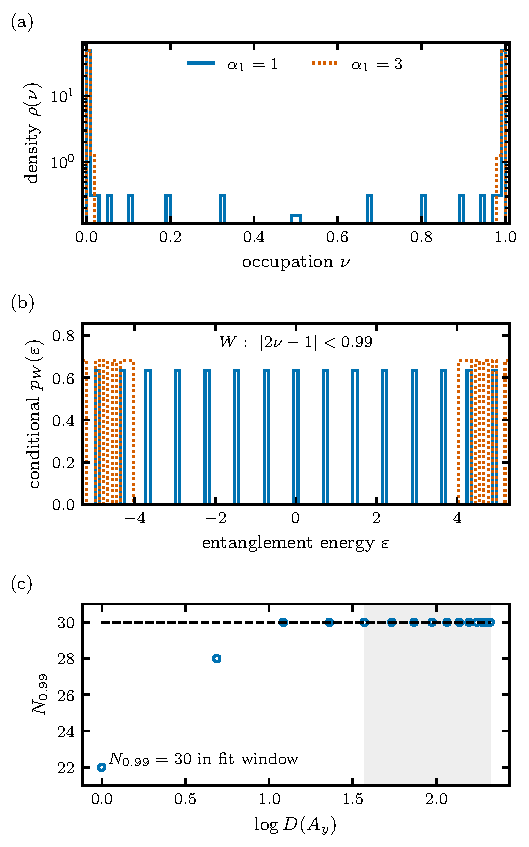
\includegraphics[width=0.5\textwidth]{Parent_07_spectrum.pdf}
\caption{Counterpart of manuscript Figure 7 at $20\times32$.
(a) Full occupation density, with zero-height bins omitted on the logarithmic
axis. (b) Conditional entanglement-energy density within $W$.
(c) Raw $\alpha_1=1$ window count versus log chord, with every strip width
$1\leq A_y\leq16$ displayed. The shaded $5\leq A_y\leq16$ fit gives the
constant 30. No ensemble broadening or statistical error bars are introduced.}
\end{figure}

\clearpage
\section{Entropy carried by each wall: manuscript Figure 8}
The additive Gaussian entropy contour of the full strip is
\begin{equation}
 s(x,\delta y)=\sum_{\mu,a}|u_a(x,\delta y,\mu)|^2h(\nu_a),\qquad
 \sum_{x,\delta y}s(x,\delta y)=S(A_y).
\end{equation}
We integrate over the two-column windows $x=5,6$ and $x=14,15$.
These are contributions to the full-strip entropy, not entropies of separately
traced narrow strips. With the same half-strip subtraction as above, the slopes
are $m_L=\LeftSlope$ and $m_R=\RightSlope$, giving
\begin{equation}
 3m_L=\LeftWeight,\qquad 3m_R=\RightWeight.
\end{equation}
Each wall contributes nearly one half of the full-strip coefficient. Equality
of the two clean-parent values contrasts with the small asymmetry of the sampled
trajectory curves. The leading coefficient carried outside these windows is small
but need not vanish exactly. Entropy weights alone do not fix chirality.

\begin{figure}[htbp]
\centering
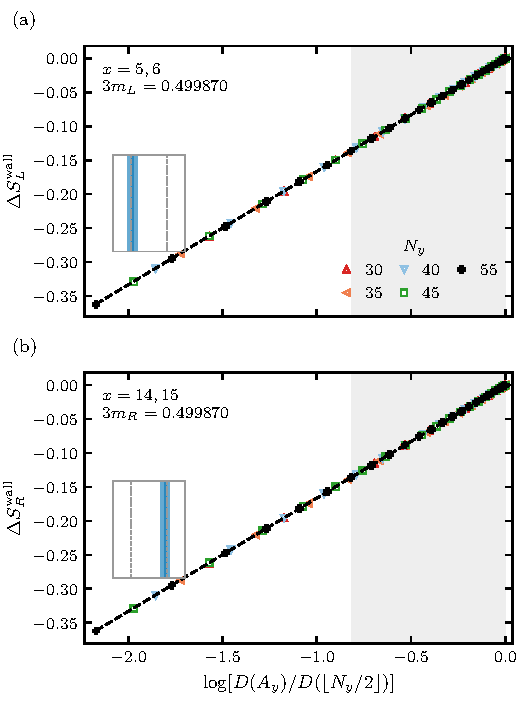
\includegraphics[width=0.5\textwidth]{Parent_08_wall_entropy.pdf}
\caption{Counterpart of manuscript Figure 8. Half-strip-subtracted contour sums
for (a) the left window $x=5,6$ and (b) the right window $x=14,15$, at
$N_y=30,35,40,45,55$, $N_x=20$, and $\alpha_1=1$. Insets mark the two integrated
columns. Joint fits use $8\leq A_y\leq\lfloor N_y/2\rfloor$ and equal total
weight per size; displayed widths begin at two.}
\end{figure}

\clearpage
\section{Modular evolution: manuscript Figure 9}
For a half-strip, use the manuscript correlation convention to define
\begin{equation}
 h_A=\log[(\Id-G_A)G_A^{-1}],\qquad
 \varphi(t_{\mathrm{mod}})=\ee^{-\ii h_A^{\mathsf T}t_{\mathrm{mod}}}\varphi(0).
\end{equation}
Since $G_A=P_A^{\mathsf T}$, the calculation diagonalizes $P_A$ and propagates
with its entanglement energies. This explicitly preserves the transpose in the
annihilation-profile convention. Centered occupations are clipped to
$\pm(1-\epsilon)$ with $\epsilon=10^{-10}$ for the primary figure.

At each source $(x_s,\delta y)=(5,8),(15,8)$, the two orbital basis profiles are
evolved separately and their densities added incoherently, with total norm two.
The displacement uses the retained weight in the five-column source window:
\begin{equation}
 \Delta y_{x_s}(t_{\mathrm{mod}})=
 \frac{\sum_{x=x_s-2}^{x_s+2}\sum_{\delta y=0}^{15}
 (\delta y-8)p_{x_s}(x,\delta y;t_{\mathrm{mod}})}
 {\sum_{x=x_s-2}^{x_s+2}\sum_{\delta y=0}^{15}p_{x_s}(x,\delta y;t_{\mathrm{mod}})}.
\end{equation}
The topological state's two displacements have opposite signs for all three
cutoffs $10^{-8},10^{-10},10^{-12}$. Their magnitudes and oscillations are cutoff
dependent: changing the cutoff shifts the curves by up to approximately $0.26$
lattice cells over the displayed interval. The trivial displacement remains
below $1.2\times10^{-6}$ across these checks. Modular time is not circuit time;
these curves diagnose handedness rather than a circuit transport velocity.

\begin{figure}[htbp]
\centering
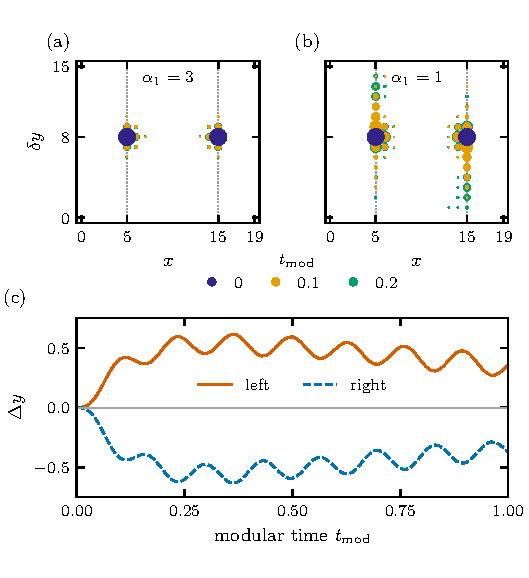
\includegraphics[width=0.5\textwidth]{Parent_09_modular.pdf}
\caption{Counterpart of manuscript Figure 9 at $20\times32$, $A_y=16$.
Density snapshots at $t_{\mathrm{mod}}=0,0.1,0.2$ for (a) $\alpha_1=3$ and
(b) $\alpha_1=1$. Marker areas follow the manuscript's density encoding.
(c) Left- and right-wall displacements for $\alpha_1=1$, sampled every 0.01.
The primary cutoff is $10^{-10}$; no SEM bands are applicable.}
\end{figure}

\clearpage
\section{Spatial contour and mutual information: manuscript Figure A2}
The topological contour contains weight along the walls in addition to the
entanglement cuts. The trivial contour is concentrated near the cuts. For the
mutual-information comparison, take opposite full-width strips $a,b$, each of
width $\ell=N_y/4$, and compute
\begin{equation}
 I_{a,b}=S(a)+S(b)-S(a\cup b).
\end{equation}
Translation symmetry makes all distinct strip placements equivalent. The
continuum two-interval reference retained from the manuscript is
$I_{a,b}=(\log2)/3$ for a unit free-fermion coefficient at this cross ratio.
The deterministic parameter scan uses the exact nonuniform 21-point manuscript
grid, including $\alpha_1=2$. At that point the zero Bloch vector is assigned
$P_+(0)=P_-(0)=\Id/2$ by the canonical construction; an open black ring identifies
that explicitly prescribed point rather than interpolating through it silently.

\begin{figure}[htbp]
\centering
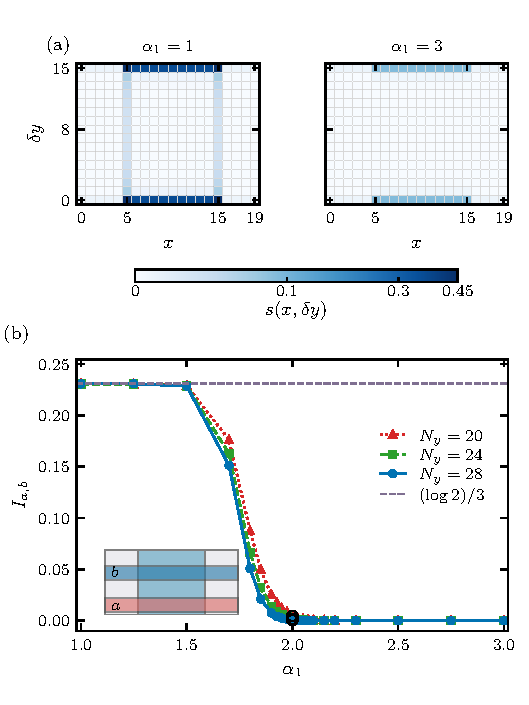
\includegraphics[width=0.5\textwidth]{Parent_A2_contour_mi.pdf}
\caption{Counterpart of manuscript Figure A2. (a) Ground-state half-strip entropy
contours at $20\times32$, $A_y=16$, for $\alpha_1=1,3$, with a shared square-root
color scale. (b) Antipodal mutual information for $N_y=20,24,28$ and $N_x=20$.
The dashed line is $(\log2)/3$; lines connect sampled parameters. The inset
identifies the two separated strips. All results are from the clean periodic
parent at exact half filling.}
\end{figure}

\clearpage
\section{Numerical validation and interpretation}
The result bundle contains 79 deterministic configurations, source and
configuration hashes, all plotted arrays, and CSV tables. Direct dense assembly
on a small lattice validates the momentum-block construction against the signed
OW sum. Additional checks cover projector rank and idempotency, translation
symmetry, hard-wall separation, Chern signs, the finite marker sum rule, Gaussian
entropy and charge identities, normalized histograms, and modular norm
conservation. A small exact Fock-space calculation independently verifies the
factor of two and transpose in Eq.~\eqref{eq:filter}.

The earlier equilibrium density benchmark used a $10^{-7}$ shift of the momentum
argument of representative OW columns before reconstruction in the untwisted
periodic basis. Repeating that prescription on the same $20\times30$ input gives
$g_{\mathrm{hf}}=\RegulatedGap$, compared with $\PeriodicGap$ here. This is a
protocol difference: the new benchmark retains the strictly periodic parent
requested for this note. The earlier periodic $20\times60$ wall analysis is
separately reproduced on its saved projector and correlator data; its cotangent
fit explains why the present antipodal chord fit does not collapse.

The requested comparisons separate three conclusions. First, bulk topology,
unit entropy and charge coefficients, equal half-unit wall entropy weights, and
opposite modular handedness have close clean equilibrium counterparts. Second,
the periodic lowest gap and the antipodal correlation shape depend on the
finite-system boundary sector and the observable used. Third, the clean
restricted spectrum is discrete, so a hard window count can plateau even while
entropy varies logarithmically. These distinctions should remain visible if the
benchmarks are later incorporated into an appendix.

\subsection{Reproduction}
Run the local CPU scripts from this directory:
\begin{verbatim}
python benchmark.py --threads 4
python analyze.py --threads 4
python validate.py --threads 4
python render.py
latexmk -pdf -interaction=nonstopmode -halt-on-error \
  -outdir=build parent_hamiltonian_benchmark_figs.tex
python verify.py --record
\end{verbatim}
The final verifier copies the successfully built PDF to this directory and records
the delivered files. Per-configuration NPZ/JSON pairs allow verified completed
calculations to be reused. Invalid source identities or checksums trigger
recomputation. Figure typography uses the existing manuscript style with this
note's own inclusion widths and output directory. No circuit simulations, cloud
jobs, or manuscript figure replacements are involved.
\end{document}
